 \documentclass[journal,12pt,twocolumn]{IEEEtran}

\usepackage{setspace}
\usepackage{gensymb}
\singlespacing
\usepackage[cmex10]{amsmath}

\usepackage{amsthm}
\usepackage{commath}
\usepackage{mathrsfs}
\usepackage{txfonts}
\usepackage{stfloats}
\usepackage{bm}
\usepackage{cite}
\usepackage{cases}
\usepackage{subfig}

\usepackage{longtable}
\usepackage{multirow}

\usepackage{enumitem}
\usepackage{mathtools}
\usepackage{steinmetz}
\usepackage{tikz}
\usepackage{circuitikz}
\usepackage{verbatim}
\usepackage{tfrupee}
\usepackage[breaklinks=true]{hyperref}
\usepackage{graphicx}
\usepackage{tkz-euclide}

\usetikzlibrary{calc,math}
\usepackage{listings}
    \usepackage{color}                                            %%
    \usepackage{array}                                            %%
    \usepackage{longtable}                                        %%
    \usepackage{calc}                                             %%
    \usepackage{multirow}                                         %%
    \usepackage{hhline}                                           %%
    \usepackage{ifthen}                                           %%
    \usepackage{lscape}     
\usepackage{multicol}
\usepackage{chngcntr}

\DeclareMathOperator*{\Res}{Res}

\renewcommand\thesection{\arabic{section}}
\renewcommand\thesubsection{\thesection.\arabic{subsection}}
\renewcommand\thesubsubsection{\thesubsection.\arabic{subsubsection}}

\renewcommand\thesectiondis{\arabic{section}}
\renewcommand\thesubsectiondis{\thesectiondis.\arabic{subsection}}
\renewcommand\thesubsubsectiondis{\thesubsectiondis.\arabic{subsubsection}}
\newtheorem{theorem}{Theorem}[section]
\newtheorem{corollary}{Corollary}[theorem]
\newtheorem{lemma}[theorem]{Lemma}
\newtheorem{definition}{Definition}[section]

\hyphenation{op-tical net-works semi-conduc-tor}
\def\inputGnumericTable{}                                 %%

\lstset{
%language=C,
frame=single, 
breaklines=true,
columns=fullflexible
}
\begin{document}

\newcommand{\BEQA}{\begin{eqnarray}}
\newcommand{\EEQA}{\end{eqnarray}}
\newcommand{\define}{\stackrel{\triangle}{=}}
\bibliographystyle{IEEEtran}
\raggedbottom
\setlength{\parindent}{0pt}
\providecommand{\mbf}{\mathbf}
\providecommand{\pr}[1]{\ensuremath{\Pr\left(#1\right)}}
\providecommand{\qfunc}[1]{\ensuremath{Q\left(#1\right)}}
\providecommand{\sbrak}[1]{\ensuremath{{}\left[#1\right]}}
\providecommand{\lsbrak}[1]{\ensuremath{{}\left[#1\right.}}
\providecommand{\rsbrak}[1]{\ensuremath{{}\left.#1\right]}}
\providecommand{\brak}[1]{\ensuremath{\left(#1\right)}}
\providecommand{\lbrak}[1]{\ensuremath{\left(#1\right.}}
\providecommand{\rbrak}[1]{\ensuremath{\left.#1\right)}}
\providecommand{\cbrak}[1]{\ensuremath{\left\{#1\right\}}}
\providecommand{\lcbrak}[1]{\ensuremath{\left\{#1\right.}}
\providecommand{\rcbrak}[1]{\ensuremath{\left.#1\right\}}}
\theoremstyle{remark}
\newtheorem{rem}{Remark}
\newcommand{\sgn}{\mathop{\mathrm{sgn}}}
\providecommand{\abs}[1]{\vert#1\vert}
\providecommand{\res}[1]{\Res\displaylimits_{#1}} 
\providecommand{\norm}[1]{\lVert#1\rVert}
%\providecommand{\norm}[1]{\lVert#1\rVert}
\providecommand{\mtx}[1]{\mathbf{#1}}
\providecommand{\mean}[1]{E[ #1 ]}
\providecommand{\fourier}{\overset{\mathcal{F}}{ \rightleftharpoons}}
%\providecommand{\hilbert}{\overset{\mathcal{H}}{ \rightleftharpoons}}
\providecommand{\system}{\overset{\mathcal{H}}{ \longleftrightarrow}}
	%\newcommand{\solution}[2]{\textbf{Solution:}{#1}}
\newcommand{\solution}{\noindent \textbf{Solution: }}
\newcommand{\cosec}{\,\text{cosec}\,}
\providecommand{\dec}[2]{\ensuremath{\overset{#1}{\underset{#2}{\gtrless}}}}
\newcommand{\myvec}[1]{\ensuremath{\begin{pmatrix}#1\end{pmatrix}}}
\newcommand{\mydet}[1]{\ensuremath{\begin{vmatrix}#1\end{vmatrix}}}

\numberwithin{equation}{subsection}
\makeatletter
\@addtoreset{figure}{problem}
\makeatother
\let\StandardTheFigure\thefigure
\let\vec\mathbf
\renewcommand{\thefigure}{\theproblem}
\def\putbox#1#2#3{\makebox[0in][l]{\makebox[#1][l]{}\raisebox{\baselineskip}[0in][0in]{\raisebox{#2}[0in][0in]{#3}}}}
     \def\rightbox#1{\makebox[0in][r]{#1}}
     \def\centbox#1{\makebox[0in]{#1}}
     \def\topbox#1{\raisebox{-\baselineskip}[0in][0in]{#1}}
     \def\midbox#1{\raisebox{-0.5\baselineskip}[0in][0in]{#1}}
\vspace{3cm}
\title{Quiz 2}
\author{MANIKANTA VALLEPU \\ AI20BTECH11014}
\maketitle
\newpage
\bigskip
\renewcommand{\thefigure}{\theenumi}
\renewcommand{\thetable}{\theenumi}
Download all python codes from 
\begin{lstlisting}
https://github.com/AI20BTECH11014/EE3900-Linear-Systems-and-Signal-processing/blob/main/QUIZ_2/QUIZ_2.py
\end{lstlisting}
%
and latex-tikz codes from 
%
\begin{lstlisting}
https://github.com/AI20BTECH11014/EE3900-Linear-Systems-and-Signal-processing/blob/main/Assignment_1/Assignment_1.tex
\end{lstlisting}
%
\section{Question}
For each of the following pairs of input and output Z-transforms $X\brak{z}$ and $Y\brak{z}$,determine the region of convergence for the system function $H\brak{z}$ : 
\begin{align}
    X\brak{z} &= \dfrac{1}{1+ \frac{1}{3}z^{-1}} ,\ &\abs{z} < \frac{1}{3} \label{a}\\
    Y\brak{z} &= \dfrac{1}{\brak{1- \frac{1}{6}z^{-1}}\brak{1+ \frac{1}{3}z^{-1}}}, \ &\frac{1}{6} < \abs{z} < \frac{1}{3} \label{b}
\end{align}
\section{Solution}
we know that the z- transform of the system function $H\brak{z}$ is given by 
\begin{align}
H\brak{z} = \dfrac{Y\brak{z}}{X\brak{z}}
\end{align}
from \eqref{a} and \eqref{b},
\begin{align}
H\brak{z} &= \dfrac{\dfrac{1}{\brak{1- \frac{1}{6}z^{-1}}\brak{1+ \frac{1}{3}z^{-1}}}}{\dfrac{1}{1+ \frac{1}{3}z^{-1}}}\\
&=\dfrac{1}{1- \frac{1}{6}z^{-1}}\\
\text{The pole of this expression is $\frac{1}{6}$}
\end{align}
from \eqref{a},
\begin{align}
 X\brak{z} &= \dfrac{1}{1+ \frac{1}{3}z^{-1}}
\end{align}
with ROC $\abs{z} < \frac{1}{3}$. We shall call this ROC$_1$.
from \eqref{b},
\begin{align}
Y\brak{z} &= \dfrac{1}{\brak{1- \frac{1}{6}z^{-1}}\brak{1+ \frac{1}{3}z^{-1}}}
\end{align}
with ROC $\frac{1}{6} < \abs{z} < \frac{1}{3}$. We shall call this ROC$_2$.The ROC of the given expression will be the intersection of ROC$_1$ and ROC$_2$. Therefore, the ROC of the given sequence is $\frac{1}{6} < \abs{z}$.
$\therefore$The Z-transform of the system function $H\brak{z}$ is given by 
 \begin{align}
H\brak{z} =\dfrac{1}{1- \frac{1}{6}z^{-1}}
\end{align}
with ROC $ \abs{z} > \frac{1}{6}  $.
%
\begin{figure}[!h]
         \centering
         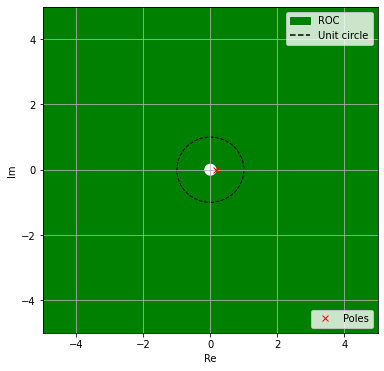
\includegraphics[width=\columnwidth]{fig_1.png}
         \caption{ Line between two points}
         \label{plot}
\end{figure}
\end{document}